% Q&A preparation for the ASHG 2026 poster. Build: ASHG/build.sh (after `python ASHG/QnA/make_tables.py`).
% Every number in the text is a macro from results/qna/numbers.tex and every table a snippet from
% results/qna/ (ASHG/QnA/make_tables.py); figures come from results/figures/ (R/make_figures.R,
% R/poster_figures.R).
\documentclass[11pt]{article}
\usepackage[letterpaper, margin=1in]{geometry}
\usepackage[T1]{fontenc}
\usepackage[default]{sourcesans}
\usepackage{amsmath, amssymb}
\usepackage{graphicx, booktabs, array, tabularx, enumitem, xcolor, float}
\usepackage{tcolorbox}
\tcbuselibrary{skins, breakable}
\usepackage[hidelinks]{hyperref}
% Relationship-type colours shared by the pedigrees and the poster (Okabe-Ito, colour-blind safe).
\definecolor{cFull}{HTML}{0072B2}   % full siblings
\definecolor{cHalf}{HTML}{009E73}   % half-siblings
\definecolor{cStep}{HTML}{D55E00}   % step-siblings
\definecolor{cAdopt}{HTML}{56B4E9}  % adoptive siblings
\definecolor{cCous}{HTML}{CC79A7}   % 1st cousins
\definecolor{cCoc}{HTML}{E69F00}    % co-cousins
\definecolor{ink}{HTML}{1F2328}
% Variance-component colours, as in the stacked bar plots (fill; darker shade for text)
\definecolor{cAdd}{HTML}{4C8CB5}   \definecolor{cAddText}{HTML}{1F4E6E}   % additive (A)
\definecolor{cGxG}{HTML}{E3894B}   \definecolor{cGxGText}{HTML}{9A4A14}   % GxG
\definecolor{cFam}{HTML}{6FAF7A}   \definecolor{cFamText}{HTML}{2F6B3A}   % family environment

\definecolor{navy}{HTML}{1F3A5F}
\definecolor{teal}{HTML}{00A1B0}
\definecolor{salmon}{HTML}{E8685F}
\graphicspath{{../../results/figures/}}
\newcommand{\res}{../../results/qna}
\makeatletter   % expandable \input, for table rows followed by \bottomrule
\newcommand{\tabinput}[1]{\@@input #1 }
\makeatother
\input{\res/numbers.tex}

\makeatletter   % navy section headings (plain LaTeX; titlesec is not installed)
\renewcommand\section{\@startsection{section}{1}{\z@}{-2.6ex \@plus -1ex \@minus -.2ex}{1.4ex \@plus .2ex}{\color{navy}\Large\bfseries}}
\renewcommand\subsection{\@startsection{subsection}{2}{\z@}{-2.2ex \@plus -1ex \@minus -.2ex}{1ex \@plus .2ex}{\color{navy}\large\bfseries}}
\makeatother
\setlist[itemize]{leftmargin=1.2em, itemsep=0.15em, topsep=0.3em}
\setlength{\parindent}{0pt}
\setlength{\parskip}{0.45em}
\frenchspacing

% one question: short answer (what to say) and the details behind it
\newcommand{\short}[1]{\begin{tcolorbox}[colback=navy!5, colframe=navy, boxrule=0.6pt, arc=2pt,
  left=6pt, right=6pt, top=4pt, bottom=4pt, title={\small\bfseries Short answer}, fonttitle=\color{white},
  coltitle=white, colbacktitle=navy]#1\end{tcolorbox}}
\newcommand{\pressed}{\par\smallskip{\color{navy}\bfseries If pressed.}\ }
\newcommand{\VG}{V_{\mathrm{GxG}}}
\newcommand{\mAGC}{A+GxG+C}

\begin{document}

\begin{center}
  {\color{navy}\LARGE\bfseries ASHG 2026 poster: questions and answers\par}
  \vspace{0.4em}
  {\large Preparation notes for Nuno R.\,G.\ Carvalho\par}
  \vspace{0.2em}
  {\small\color{gray!60!black} ``Relatives' similarity in test score performance is explained by a wide range of genetic and
  environmental parameters'', with Alexander Gusev. ASHG 2026 Annual Meeting, Montr\'eal.\par}
\end{center}

\begin{tcolorbox}[colback=salmon!8, colframe=salmon!80!black, boxrule=0.8pt, arc=2pt,
  title={\bfseries AI disclosure}, colbacktitle=salmon!80!black, coltitle=white]
These questions and answers were written by Claude (Anthropic's AI model, Opus 5.5), not by Nuno. They are
meant to help Nuno prepare to answer questions at the poster: each answer is a suggestion of what could be
said and of the evidence behind it, not a statement of the authors' conclusions, and nothing here has been
peer reviewed. The numbers are generated directly from the analysis results by
\texttt{ASHG/QnA/make\_tables.py}, but the selection of questions, the wording and the interpretation are the
AI's. Check anything before relying on it, and say it in your own words.
\end{tcolorbox}

\tableofcontents
\newpage

%=====================================================================================================
\section{How to use these notes}
Each question has a \textbf{short answer}, roughly what to say first, followed by the details to use
\textbf{if pressed}, with the figure or table that backs them up. Section~\ref{sec:feedback} goes through the
professor's feedback on the poster and points to the answers; Section~\ref{sec:questions} has the questions an
audience is likely to ask. Notation as on the poster: A (additive, with assortative mating), GxG (pairwise
gene--gene interactions), C (shared environment); ``+'' means fitted jointly, ``$\to$'' fitted in steps.

\subsection{The 30-second pitch}
Framed as a new approach rather than a correction (Section~\ref{sec:feedback}):
\short{%
Families resemble each other in test scores, and \emph{how} that resemblance falls off from twins to second
cousins and in-laws tells you about genes and shared environment. We built a \textbf{revised estimator} for
fitting these models to the correlations of $\sim$80 kinds of relatives in Norway: it fits correlations on
their natural scale, with correct weights, and can give every \emph{type} of relative equal weight so that
millions of cousin pairs don't drown out the twins. With it, the additive model gives $V_A \approx
\VARevType$ instead of the published $\VAEft$, and fits far better. Adding gene--gene interactions and
shared environment improves out-of-sample prediction, but those components trade off against each other, so
their split is poorly determined.}

\subsection{The poster in three numbers}
\begin{itemize}
  \item $V_A$ (additive model): \VAEft{} with Eftedal et al.'s estimator, \VARevType{} with the revised one
        (Marginal Type); $\chi^2/\mathrm{df}$ \ChiDfEft{} $\to$ \ChiDfRevType.
  \item Best model by cross-validation: \mAGC{}, CV RMSE \CVAGC{} vs.\ \CVA{} for the additive model.
  \item Collinearity: across leave-one-type-out refits of \mAGC, $V_A$ moves against $\VG$ ($r = \rAGCVAVG$)
        and $V_C$ ($r = \rAGCVAVC$).
\end{itemize}

%=====================================================================================================
\section{The professor's feedback}\label{sec:feedback}
The poster is printed, so the layout points (key smaller, takeaways larger, a bold headline with the
contribution) can only be addressed in how you talk about it. The content questions all have answers.

\begin{enumerate}[leftmargin=1.5em, itemsep=0.5em]
  \item \textbf{Frame the work as ``a revised estimator'', not ``problems with Eftedal's estimator''.}
        When you talk, lead with what the estimator does (natural scale, correct weights, a choice of unit:
        pairs or relative types) and present Eftedal et al.'s settings as one point in that design space.
        Useful phrasing: ``We propose a revised estimator for relatives' correlations; applied to the same
        data, it changes the additive heritability from \VAEft{} to about \VARevType.'' The poster's box
        ``Problems in Eftedal et al.'s estimator'' can be introduced as ``the design choices the revised
        estimator changes''.
  \item \textbf{Make the contribution visible in the first 10 seconds.} Open with the first two sentences of
        the pitch above, pointing at the ``Revising Eftedal et al.'s results'' panel.
  \item \textbf{Intuition for the step-sibling and weighting errors.} See Q\ref{q:weights} (weights) and
        Q\ref{q:stepsib} (step-siblings).
  \item \textbf{Show directly that the revised estimator fits better.} See Q\ref{q:fit}: $\chi^2/\mathrm{df}$
        \ChiDfEft{} $\to$ \ChiDfRevType{} and weighted $R^2$ \RsqEft{} $\to$ \RsqRevType.
  \item \textbf{Show how the fit changes as components are added.} See Q\ref{q:components}
        (Table~\ref{tab:models}).
  \item \textbf{Why \mAGC{} as the example?} See Q\ref{q:example}: it is the best model by cross-validation,
        not merely the most complex one.
  \item \textbf{Key smaller, takeaways larger.} Not changeable now; read the takeaways out when you summarise.
\end{enumerate}

%=====================================================================================================
\section{Likely questions}\label{sec:questions}

%-----------------------------------------------------------------------------------------------------
\subsection{Why does the weighting matter so much?}\label{q:weights}
\short{%
Because the weights decide which relatives the model is fitted to. Each correlation's weight $1/\mathrm{SE}^2$
is proportional to its number of pairs, so the \WeightDistantPairs\% of pairs that are 1st cousins, 2nd cousins
and co-cousins dominate. Fitting on the log scale then multiplies each weight by $1/\rho^2$: about
\WeightDistantEftEffective\% of the effective weight lands on those distant relatives and essentially none on
twins. Correcting the weights alone moves $V_A$ from \VAEft{} to \VAEftDelta.}
\pressed
\begin{itemize}
  \item \textbf{Log scale.} A residual on the log scale is roughly $(\hat\rho - \rho)/\rho$, so a miss of 0.01
        counts ten times more for a correlation of 0.05 than for 0.5. With weights $1/\mathrm{SE}^2$ the effective
        weight on the correlation scale is $1/(\mathrm{SE}^2\rho^2)$. The correct inverse variance of $\ln\hat\rho$
        is $\rho^2/\mathrm{SE}^2$ (delta method), which would cancel that factor.
  \item \textbf{Why it changes the answer.} The model is misspecified ($\chi^2/\mathrm{df} \gg 1$), so it cannot
        fit every type at once; the weights decide which compromise you get. Under Eftedal et al.'s estimator,
        leaving out the co-cousins alone moves $V_A$ from \VAEft{} to \VAEftNoCocousins{} (and leaving out full
        siblings moves it to \VAEftNoSibs).
  \item \textbf{Marginal Pair vs.\ Marginal Type.} Marginal Pair (weights $1/\mathrm{SE}^2$ on the correlation
        scale) is the correct estimator for ``a random pair of relatives''. Marginal Type gives each of the 10
        relative types equal weight: it answers ``a random kind of relative'', which is the fair basis for
        comparing models that differ in how they treat twins, siblings and in-laws.
\end{itemize}

\begin{table}[H]
\centering\small
\begin{tabular}{@{}l r r r r r@{}}
\toprule
 & & \multicolumn{2}{c}{Eftedal et al.\ (\NCategoriesEftedal{} categories)} & Marginal Pair & Marginal Type \\
\cmidrule(lr){3-4}
relative type & share of pairs & $1/\mathrm{SE}^2$ & effective (log scale) & $1/\mathrm{SE}^2$ & \\
\midrule
\tabinput{\res/t_weights.tex}
\bottomrule
\end{tabular}
\caption{Share of each fit's total weight by relative type. ``Effective'' converts Eftedal et al.'s log-scale
weights to the correlation scale ($1/(\mathrm{SE}^2\hat\rho^2)$). Eftedal et al.\ leave out the adoptive types
(and the types related through twins of unknown zygosity).}
\label{tab:weights}
\end{table}

%-----------------------------------------------------------------------------------------------------
\subsection{What was wrong with the step-sibling formula, and does it matter?}\label{q:stepsib}
\short{%
Step-siblings are related only because their parents mated assortatively. Eftedal et al.\ price every
mating step in that chain at the genetic correlation between mates, $m$; only the first step costs $m$, and
every later step costs the \emph{phenotypic} correlation $r$. The fix is
$V_A\,m\,\big((1+m)/2\big)^2 \to V_A\,m\,\big((1+r)/2\big)^2$. It matters little for $V_A$ (changes it by at
most \StepVAdiffType), but it predicts step-siblings better.}
\pressed
\begin{itemize}
  \item \textbf{The chain.} With A's parents $\{f_A, m_A\}$ and B's $\{f_B, m_B\}$, and $m_A$ mated to $f_B$,
        the parents lie on one chain $f_A - m_A - f_B - m_B$, up to three matings apart. The first crossing goes
        from a breeding value to a phenotype ($m$); every later one propagates at the phenotypic level ($r$).
  \item \textbf{Internal inconsistency.} Their own half-sibling formula, $(1+2m+rm)/4$ (Nagylaki's multiplier),
        prices a two-step crossing at $rm$; their step-sibling formula prices it at $m^2$. Both can only hold if
        $r = m$, i.e.\ $h^2 = 1$.
  \item \textbf{Size.} Since $r = m/V_A > m$, the corrected formula predicts more similarity: under the revised
        additive fit (Marginal Type) \StepPredCorrType{} vs.\ \StepPredEftType{}, against an observed
        \ObsStep. Both under-predict step-siblings.
\end{itemize}

%-----------------------------------------------------------------------------------------------------
\subsection{Does the revised estimator actually fit better?}\label{q:fit}
\short{%
Yes. Over the same model, $\chi^2/\mathrm{df}$ falls from \ChiDfEft{} to \ChiDfRevPair--\ChiDfRevType{} and the
weighted $R^2$ rises from \RsqEft{} to about \RsqRevType. Most of the gain comes from the weights alone.}
\pressed
Table~\ref{tab:corrections} applies the changes one at a time, and Figure~\ref{fig:p4} is the poster's
comparison. Caveats: each statistic is over that fit's own relationship categories (Eftedal et al.'s
\NCategoriesEftedal, ours all \NCategories), and $\chi^2$ and $R^2$ use $1/\mathrm{SE}^2$ weights, so they
favour the Marginal Pair fit by construction; no additive fit comes close to $\chi^2/\mathrm{df} \approx 1$.

\begin{table}[H]
\centering\small
\begin{tabular}{@{}l c c c c c c@{}}
\toprule
estimator & $V_A$ & 95\% CI (Marginal Type) & $m$ & $r$ & weighted $R^2$ & $\chi^2/\mathrm{df}$ \\
\midrule
\tabinput{\res/t_corrections.tex}
\bottomrule
\end{tabular}
\caption{The additive model, from Eftedal et al.'s estimator to the revised one. Rows 2--3 change one design
choice each; rows 4--5 apply all of them (correlation scale, correct weights, $m = V_A r$, corrected
step-sibling formula, all relative types). CIs are clipped to $[0, 1]$.}
\label{tab:corrections}
\end{table}

\begin{figure}[H]
\centering
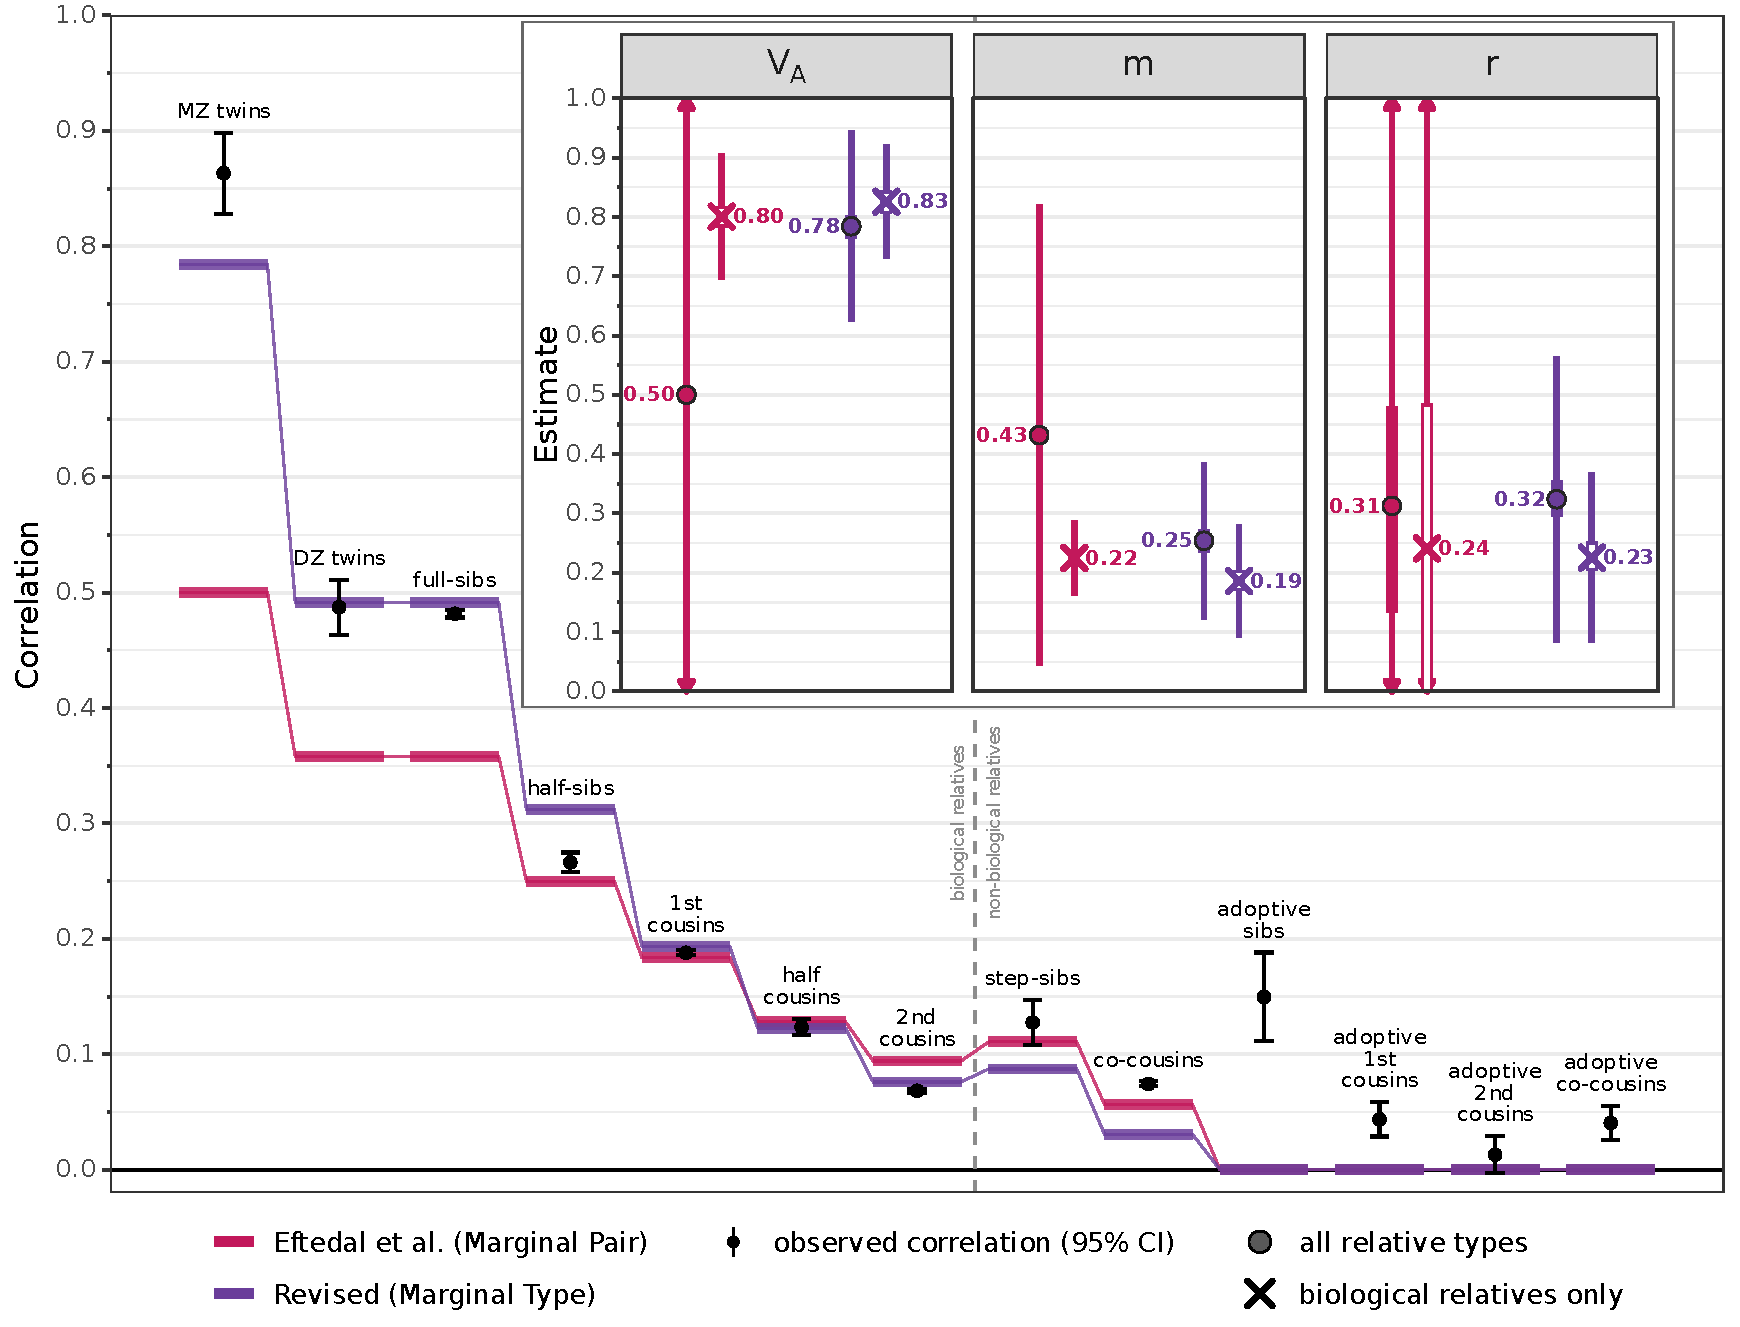
\includegraphics[width=0.78\textwidth]{poster/p4_fit_and_params}
\caption{The poster's additive-model panel: predicted correlation per relative type under Eftedal et al.'s
estimator and the revised one (Marginal Type), with the parameter estimates by training cohort.}
\label{fig:p4}
\end{figure}

%-----------------------------------------------------------------------------------------------------
\subsection{Do in-laws still pull heritability down?}\label{q:inlaw}
\short{%
No. That was a headline of Eftedal et al.: $h^2$ drops from \InlawBioEft{} to \InlawAllEft{} when in-laws are
added. With the revised estimator the drop is \InlawDiffRevType{} (Marginal Type, 95\% CI
[\InlawDiffLoRevType, \InlawDiffHiRevType]). Their own 0.30 gap has a Marginal Type CI of
[\InlawDiffLoEft, \InlawDiffHiEft]: it hinges on the co-cousin type.}
\pressed
The Marginal Pair intervals in Table~\ref{tab:inlaw} make every difference look ``significant'' because they
count sampling noise only; the Marginal Type interval asks whether the difference survives leaving out one
relative type. The in-law categories still fit poorly (co-cousins are under-predicted), but with a correct
estimator they no longer pull $h^2$ down; the same holds for all 13 tests in the data set (notebook, S6).

\begin{table}[H]
\centering\small
\begin{tabular}{@{}l c c c c c@{}}
\toprule
 & \multicolumn{2}{c}{$h^2$} & & \multicolumn{2}{c}{95\% CI of the difference} \\
\cmidrule(lr){2-3}\cmidrule(lr){5-6}
estimator & biological only & + in-laws & difference & Marginal Type & Marginal Pair \\
\midrule
\tabinput{\res/t_inlaw.tex}
\bottomrule
\end{tabular}
\caption{Additive-model $h^2$ fitted to biological relatives only and with in-laws (step-siblings and
co-cousins). CIs on the difference are paired: the same relative type is left out of both fits.}
\label{tab:inlaw}
\end{table}

%-----------------------------------------------------------------------------------------------------
\subsection{Do GxG and shared environment improve the fit?}\label{q:components}
\short{%
Jointly fitted, yes: \mAGC{} has $\chi^2/\mathrm{df}$ \ChiDfModelAGC{} against \ChiDfModelA{} for the additive
model, and the best cross-validation error (\CVAGC{} vs.\ \CVA). Added in a second step on top of a fixed
additive fit, they barely help, because the additive part has already absorbed the shared signal.}
\pressed
Table~\ref{tab:models} has every core model. A$\to$C is even worse than A by $\chi^2/\mathrm{df}$: its second
step ends with $c = 0$, a term shared by siblings only. The sum of the components is well determined
(\VsumMin--\VsumMax{} across models); the split is not (Q\ref{q:collinear}).

\begin{table}[H]
\centering\small
\begin{tabular}{@{}l c c c c c c c@{}}
\toprule
 & & & \multicolumn{3}{c}{cross-validation} & \multicolumn{2}{c}{without adoptive types} \\
\cmidrule(lr){4-6}\cmidrule(lr){7-8}
model & weighted $R^2$ & $\chi^2/\mathrm{df}$ & CV RMSE & rank & SE behind best & CV RMSE & adoptive share \\
\midrule
\tabinput{\res/t_models.tex}
\bottomrule
\end{tabular}
\caption{The nine core models (Marginal Type fit). ``SE behind best'': the paired difference in CV score from
\mAGC, in standard errors over the 10 held-out types. ``Adoptive share'': the adoptive types' share of the
model's CV score.}
\label{tab:models}
\end{table}

\begin{figure}[H]
\centering
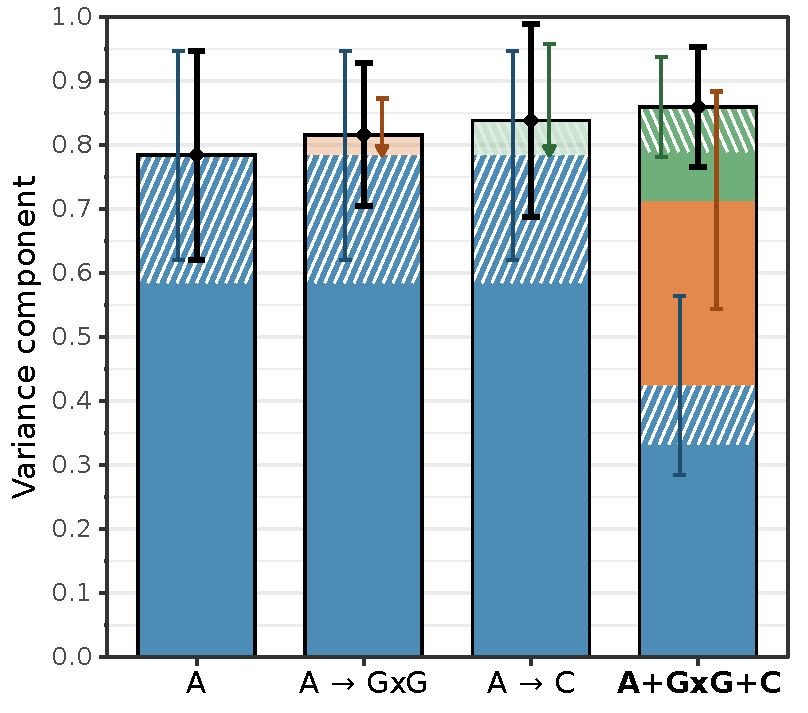
\includegraphics[width=0.5\textwidth]{poster/p6_components_four_models}
\caption{The poster's variance components for A, A$\to$GxG, A$\to$C and \mAGC.}
\end{figure}

%-----------------------------------------------------------------------------------------------------
\subsection{Why \mAGC{} as the example? Is it the best model?}\label{q:example}
\short{%
It is the best model by leave-one-type-out cross-validation (rank 1 of 9, CV RMSE \CVAGC), and stays best
when the adoptive types are left out (\CVnoadAGC). Being the most complex model doesn't guarantee that:
A$\to$GxG+C has the same three components and ranks last. But the margin is modest: about \ZA{} standard errors
ahead of the additive model and \ZAC{} ahead of A+C.}
\pressed
Cross-validation predicts each relative type from a fit to the other nine, so a model only wins by
generalising across kinds of relatives (Figures~\ref{fig:cv} and \ref{fig:cvtype}). The additive model is worse
in \FoldsWorseA{} of the 10 held-out types.

\begin{figure}[H]
\centering
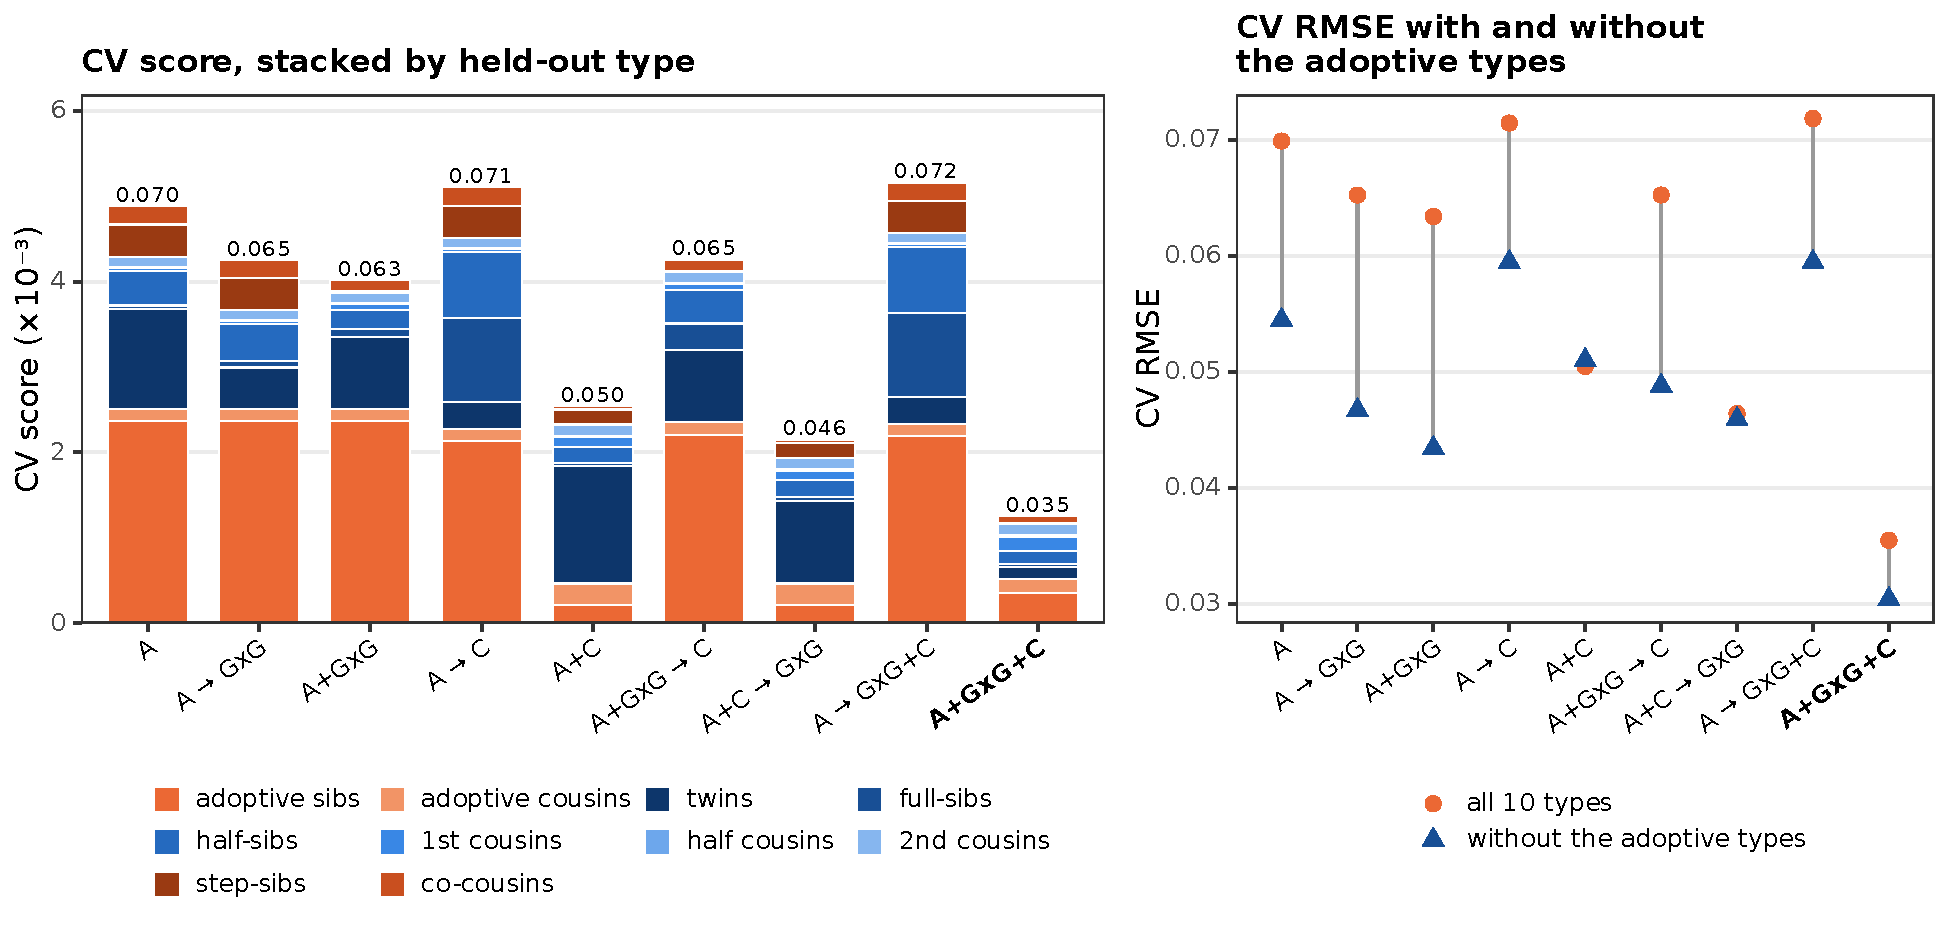
\includegraphics[width=0.9\textwidth]{poster/supplement/s_cv_by_type}
\caption{Where each model's cross-validation error comes from (left), and CV RMSE with and without the
adoptive types (right).}
\label{fig:cvtype}
\end{figure}

%-----------------------------------------------------------------------------------------------------
\subsection{Isn't GxG just standing in for shared environment (or vice versa)?}\label{q:collinear}
\short{%
Partly, and that is the poster's point: they are collinear. Across the leave-one-type-out refits of \mAGC,
$V_A$ moves against $\VG$ ($r = \rAGCVAVG$) and against $V_C$ ($r = \rAGCVAVC$), and in two-step fits whichever
component comes first takes the shared signal ($\VG$ is \VGAtoG{} after A, \VGAG{} jointly). But they are not
interchangeable: GxG captures the steep fall-off from twins to siblings, and C the similarity of adoptees.}
\pressed
Without the adoptive types, A+GxG predicts better than A+C (CV RMSE \CVnoadAG{} vs.\ \CVnoadAC); with them,
A+C wins, entirely through the adoptive siblings. \mAGC{} is best either way, so each component explains
something the other cannot. Figure~\ref{fig:pairs} shows the trade-offs.

\begin{figure}[H]
\centering
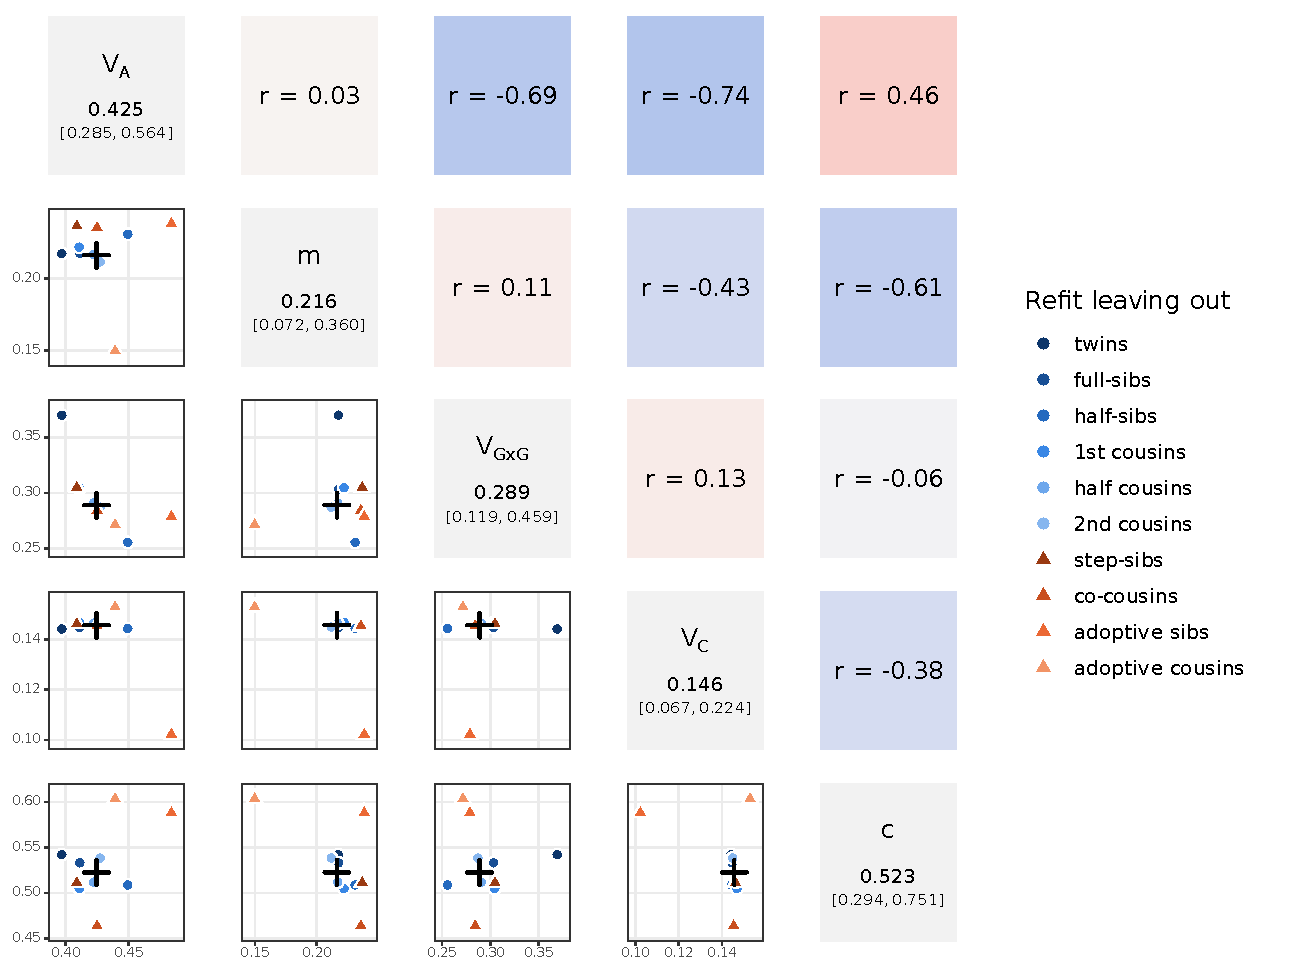
\includegraphics[width=0.75\textwidth]{poster/supplement/s_paircorr_AGxGF}
\caption{\mAGC: estimates from the 10 leave-one-type-out refits (lower), their correlation (upper), and each
estimate with its Marginal Type CI (diagonal).}
\label{fig:pairs}
\end{figure}

%-----------------------------------------------------------------------------------------------------
\subsection{What about the adoptees?}\label{q:adoptees}
\short{%
They are the clearest evidence for shared environment. Adoptive siblings correlate about \ObsAdoptSibs,
but any genetics-only model predicts exactly 0 for them; adoptive types make up \AdShareA\% of the additive
model's cross-validation error. Only models with a jointly fitted C reach them.}
\pressed
Two-step C models estimate $c = 0$, so their C is a within-sibling term of about 0.05: they still
under-predict adoptive siblings and over-predict biological siblings. With C fitted jointly, adoptive cousins
are slightly over-predicted. Figure~\ref{fig:cv} shows each model's mean residual by held-out type; hatched
tiles are types the model predicts to be 0.

\begin{figure}[H]
\centering
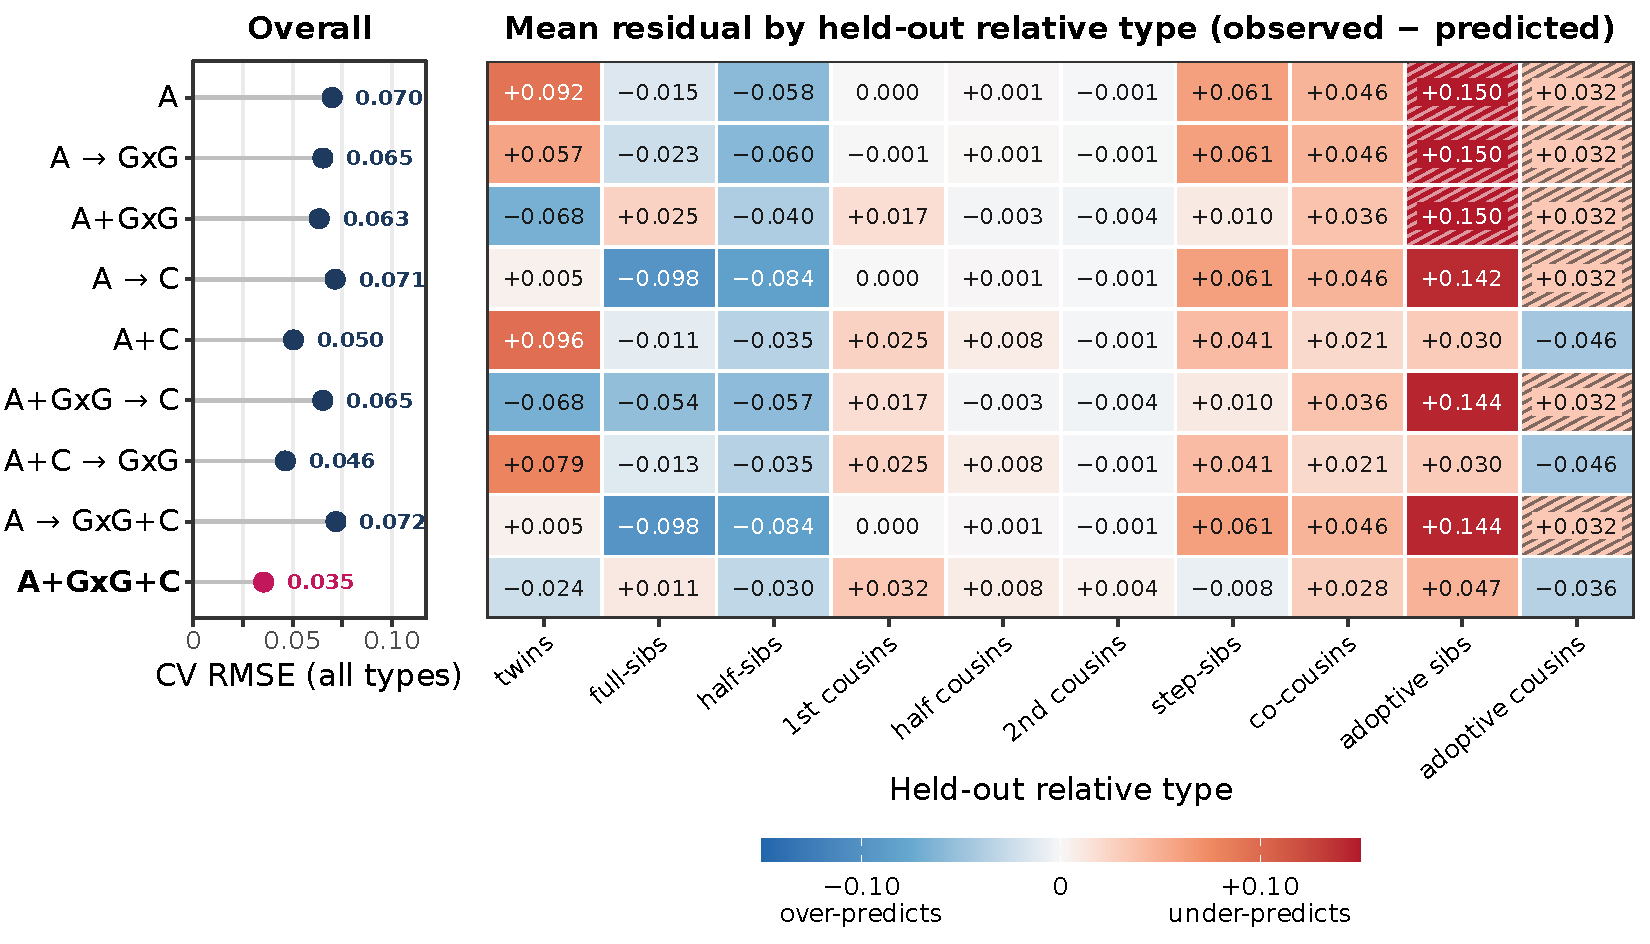
\includegraphics[width=0.85\textwidth]{poster/supplement/s_cv}
\caption{Cross-validation: overall CV RMSE (left) and the mean residual, observed $-$ predicted, of each
held-out relative type (right).}
\label{fig:cv}
\end{figure}

%-----------------------------------------------------------------------------------------------------
\subsection{How should $V_A$ be read under assortative mating?}\label{q:am}
\short{%
$V_A$ is the additive variance in today's population, inflated by assortative mating. The variance it would
have under random mating is $V_A^0 = V_A(1-m)$: \VAzeroRevType{} against $V_A = \VARevType$ in the revised
additive model ($m = \mRevType$, $r = \rRevType$).}
\pressed
The model imposes $m = V_A\,r$ (mates' genetic correlation = heritability $\times$ their phenotypic
correlation), which Eftedal et al.\ estimated separately; it leaves the additive part two degrees of freedom.
$V_A$ and $m$ trade off ($r = \rAVAm$ across refits). In A+C the shared environment absorbs the slow decay with
distance and $m = r = 0$, which is implausible for test scores; that is one reason not to read any single
model's split literally.

%-----------------------------------------------------------------------------------------------------
\subsection{How much should we trust the intervals?}\label{q:intervals}
\short{%
The Marginal Pair interval (parametric bootstrap) is sampling noise only, and with millions of pairs it is
tiny. The Marginal Type interval (leave-one-type-out jackknife) asks how much the estimate depends on which
kinds of relatives exist; that is the uncertainty that matters for a misspecified model, so we lead with it.
It is crude (10 heterogeneous units), and unreliable for parameters estimated on a bound.}
\pressed
Both intervals are centred on the full-data estimate, which is the standard jackknife construction.
Table~\ref{tab:jackknife} checks the jackknife bias: for interior parameters it is under one SE; for
parameters on a bound ($m = r = 0$ in A+C, $c = 0$ in two-step C models) it is 1.3--1.7 SE and the symmetric
interval should not be read literally. None of the poster's intervals is of the second kind.

\begin{table}[H]
\centering\small
\begin{tabular}{@{}l c c l c r c c@{}}
\toprule
model & parameter & estimate & & mean of refits & jackknife bias & SE & $|$bias$|$/SE \\
\midrule
\tabinput{\res/t_jackknife.tex}
\bottomrule
\end{tabular}
\caption{Jackknife bias, $(B-1)(\bar\theta_{(\cdot)} - \hat\theta)$ with $B = 10$, against the jackknife SE.}
\label{tab:jackknife}
\end{table}

%-----------------------------------------------------------------------------------------------------
\subsection{How did Eftedal et al.\ get their intervals?}\label{q:eftedalci}
\short{%
Not stated in the paper, but their code reproduces Table~1 exactly: a $t$-interval from a log-linear regression
for the biological-only model, and for the headline model a bootstrap that resamples relationship categories
with probability $\propto 1/\mathrm{SE}^2$. They also computed inverse-Hessian intervals, about
\HessianNarrower{} times narrower, and did not report them.}
\pressed
Resampling in proportion to $1/\mathrm{SE}^2$ and then refitting with $1/\mathrm{SE}^2$ weights concentrates the
replicates on the distant relatives (MZ twins appear in only about 5\% of resamples), so their intervals mostly
reflect disagreement among cousin types.

\begin{table}[H]
\centering\small
\begin{tabular}{@{}p{2.3cm} p{4.6cm} c c c c@{}}
\toprule
model & method & $h^2$ & our replication & published & reported \\
\midrule
\tabinput{\res/t_eftedal_ci.tex}
\bottomrule
\end{tabular}
\caption{Eftedal et al.'s interval methods for $h^2$, reproduced from their code.}
\end{table}

%-----------------------------------------------------------------------------------------------------
\subsection{Does any model actually fit?}\label{q:misfit}
\short{%
No, and that is the third takeaway. Even the best models have $\chi^2/\mathrm{df}$ around \ChiDfMin; a correct
model would give about 1. The observed correlations sit several standard errors from every model's
predictions, because the SEs are tiny and the models miss systematic structure.}
\pressed
Overlapping pairs make the SEs too small, but Eftedal et al.\ estimate by less than 30\%, which would inflate
$\chi^2/\mathrm{df}$ by at most about 1.7. The residual patterns (Figure~\ref{fig:cv}) show what is missing:
twins and siblings for models without GxG or joint C, adoptees for models without C, and in-laws for nearly
every model.

%-----------------------------------------------------------------------------------------------------
\subsection{What are the main limitations and next steps?}\label{q:limits}
\short{%
The models are simple by design. The ones I would name: family degrees for the shared environment were
chosen by intuition, assortative mating is assumed to be at equilibrium and on the phenotype, the GxG kernel is
an idealisation, and the correlations are treated as independent.}
\pressed
\begin{itemize}
  \item \textbf{Shared environment.} The decay $c^{f}$ over a ``family degree'' $f$ is one simple form; other
        degree assignments may fit better.
  \item \textbf{Assortative mating.} Equilibrium, primary phenotypic assortment ($m = V_A r$).
  \item \textbf{GxG.} Pairwise interactions with kernel $(1/4)^n$, unaffected by assortative mating; a
        simulation check is in the repository (\texttt{theory/gxg\_kernel}).
  \item \textbf{Data.} One phenotype (mean 8th-grade test score) for the main results, with robustness checks
        across all 13 tests for the in-law contrast; correlations treated as independent.
  \item \textbf{Next.} Joint modelling of the dependence among correlations, alternative environment
        structures, and applying the revised estimator to other relative-correlation data sets.
\end{itemize}

\end{document}
